
\section{Events and Source Properties}

The 30 earthquakes considered for the evaluation of the models in this article are labeled with a sequential letter-code from A to to AD in Fig.~\ref{fig:region} with their detailed information presented in Table \ref{tab:events}  \citet{Lee_2011_GJI}.
They are a set of earthquakes which are happened between 1998 and 2014, and had magnitudes between 3.6 and 5.4, and hypocenter depths that vary between 3.6 and 21.1~km. Events are modeled as a point source analogy with rupture parameters scaled according to the magnitude of each earthquake and source time functions respecting to that.



\begin{table*}
	\centering\small
	\caption{Selected events with their ID \citet{SCEC} and description of source location, magnitude, focal mechanism (strike, dip, and rake angles) \citet{Lee_2011_GJI}, and date and time (in coordinated universal time, or UTC).}
	\begin{tabular}[t]{@{} c l r c r@{, }l r c c c r}
	\\[-3ex]
	\hline
	  	Code								& 
	  	Earthquake name						&
	  	Event ID							& 
	  	\eqmag{w}							&
	  	\multicolumn{2}{c}{Coordinates}		&
	  	Depth								&
	  	Strike/Dip/Rake						&
	  	Date								&
	  	UTC Time							&
	  	Num.								\\
	  										& 
	  										&	
	  										& 
	  										&	
	  	\multicolumn{2}{c}{(lon., lat.)} 	&
	  	(km)								&	
	  										&
	  	(yyyy/mm/dd)						&
	  	(hh:mm:ss)							&
	  	Stns.\\
	\hline																																
		A	& Wrightwood			&	 9064568	&	4.40	&	--117.6480	&	34.3740	&	 8.99	&	285/57/86	&	1998/08/20	&	23:49:58.198	&	17	\\ % A 
		B	& NW of Devore			&	10972299	&	3.79	&	--117.4642	&	34.2655	&	10.91	&	 98/58/68	&	2001/07/19	&	20:42:36.470	&	52	\\ % R
		C	& NNE of Devore			&	14494128	&	3.72	&	--117.3838	&	34.2587	&	 7.18	&	344/69/-33	&	2009/08/01	&	12:55:55.317	&	77	\\ % Z
		D	& Yucaipa				&	14155260	&	4.88	&	--117.0113	&	34.0580	&	11.61	&	 75/59/55	&	2005/06/16	&	20:53:26.225	&	172	\\ % V
																					
		E	& N of Rancho Cucamonga	&	10216101	&	3.60	&	--117.5762	&	34.2058	&	 4.92	&	 54/69/16	&	2006/11/04	&	19:43:44.376	&	55	\\ % J
																					
		F	& 2002 Fontana			&	13692644	&	3.74	&	--117.4288	&	34.1613	&	 6.54	&	233/72/-28	&	2002/07/25	&	00:43:14.872	&	55	\\ % S
		G	& 2005 Fontana			&	14116972	&	4.42	&	--117.4387	&	34.1250	&	 4.15	&	222/88/-25	&	2005/01/06	&	14:35:27.593	&	83	\\ % U
		H	& San Bernardino		&	10370141	&	4.45	&	--117.3042	&	34.1073	&	14.22	&	 87/70/28	&	2009/01/09	&	03:49:46.051	&	159	\\ % L
		I	& N of Loma Linda		&	 9140050	&	4.37	&	--117.2525	&	34.0500	&	15.36	&	270/90/-6	&	2000/02/21	&	13:49:43.017	&	38	\\ % D
		J	& Redlands				&	10541957	&	4.10	&	--117.1797	&	34.0045	&	 8.53	&	 33/46/-68	&	2010/02/13	&	21:39:06.349	&	97	\\ % Q
		K	& 2010 Beaumont			&	10530013	&	4.28	&	--117.0232	&	33.9322	&	13.93	&	234/89/9	&	2010/01/16	&	12:03:25.345	&	76	\\ % P
		L	& 2006 Beaumont			&	14239184	&	3.90	&	--117.1122	&	33.8560	&	11.53	&	 45/31/-25	&	2006/07/10	&	02:54:43.809	&	66	\\ % W
																					
		M	& Simi Valley			&	14000376	&	3.59	&	--118.7530	&	34.2722	&	13.81	&	234/62/60	&	2003/10/29	&	23:44:48.206	&	54	\\ % T
		N	& WSW of Valencia		&	 9753489	&	3.90	&	--118.6678	&	34.3705	&	14.21	&	 83/62/57	&	2002/01/29	&	06:00:39.140	&	52	\\ % H
		O	& N of Pico Canyon		&	 9096972	&	3.98	&	--118.6090	&	34.3980	&	11.53	&	287/55/54	&	1999/07/22	&	09:57:23.502	&	26	\\ % C
		P	& Chatsworth			&	14312160	&	4.66	&	--118.6195	&	34.2995	&	 7.58	&	 82/27/51	&	2007/08/09	&	07:58:48.888	&	109	\\ % X
		Q	& Newhall				&	15237281	&	3.86	&	--118.4580	&	34.3508	&	 3.59	&	236/58/33	&	2012/10/28	&	15:24:23.172	&	120	\\ % AC
																					
		R	& Beverly Hills			&	 9703873	&	4.24	&	--118.3885	&	34.0590	&	 7.90	&	262/81/4	&	2001/09/09	&	23:59:17.695	&	130	\\ % F
		S	& Inglewood Area		&	10410337	&	4.70	&	--118.3357	&	33.9377	&	13.86	&	243/60/25	&	2009/05/18	&	03:39:36.126	&	213	\\ % O
		T	& NW of Compton			&	 9716853	&	3.98	&	--118.2702	&	33.9290	&	21.13	&	116/68/71	&	2001/10/28	&	16:27:45.388	&	55	\\ % G
																					
		U	& Downtown Los Angeles	&	 9093975	&	3.77	&	--118.2180	&	34.0100	&	 9.53	&	125/49/79	&	1999/06/29	&	12:55:00.371	&	25	\\ % B
																					
		V	& Whittier Narrows		&	14601172	&	4.44	&	--118.0817	&	33.9923	&	18.85	&	282/36/73	&	2010/03/16	&	11:04:00.026	&	180	\\ % AA
		W	& La Habra				&	15481673	&	5.10	&	--117.9300	&	33.9220	&	 5.00	&	239/70/38	&	2014/03/29	&	04:09:42.970	&	311	\\ % AD
		X	& Chino Hills			&	14383980	&	5.39	&	--117.7613	&	33.9530	&	14.70	&	 47/51/32	&	2008/07/29	&	18:42:15.960	&	335	\\ % Y
		Y	& 2002 Yorba Linda		&	 9818433	&	4.75	&	--117.7758	&	33.9173	&	12.92	&	 34/84/-10	&	2002/09/03	&	07:08:51.675	&	67	\\ % I
		Z	& 2009 Yorba Linda		&	10399889	&	3.98	&	--117.7892	&	33.8940	&	 4.23	&	208/65/26	&	2009/04/24	&	03:27:49.840	&	91	\\ % M
		AA	& ESE of Yorba Linda	&	 9644101	&	3.64	&	--117.6882	&	33.8777	&	 3.59	&	 56/65/37	&	2001/04/13	&	11:50:11.916	&	53	\\ % E
																					
		AB	& Lake Elsinore			&	10275733	&	4.73	&	--117.4770	&	33.7322	&	12.60	&	 65/59/58	&	2007/09/02	&	17:29:14.827	&	116	\\ % K
																					
		AC	& Westlake Village		&	10403777	&	4.42	&	--118.8825	&	34.0667	&	14.17	&	254/73/30	&	2009/05/02	&	01:11:13.084	&	94	\\ % N
																					
		AD	& Hermosa Beach			&	14738436	&	3.69	&	--118.4578	&	33.8572	&	11.23	&	 57/41/54	&	2010/06/07	&	23:59:27.165	&	93	\\ % AB
	\hline
	\end{tabular}
	\label{tab:events}
\end{table*}




\begin{figure}
    \centering
    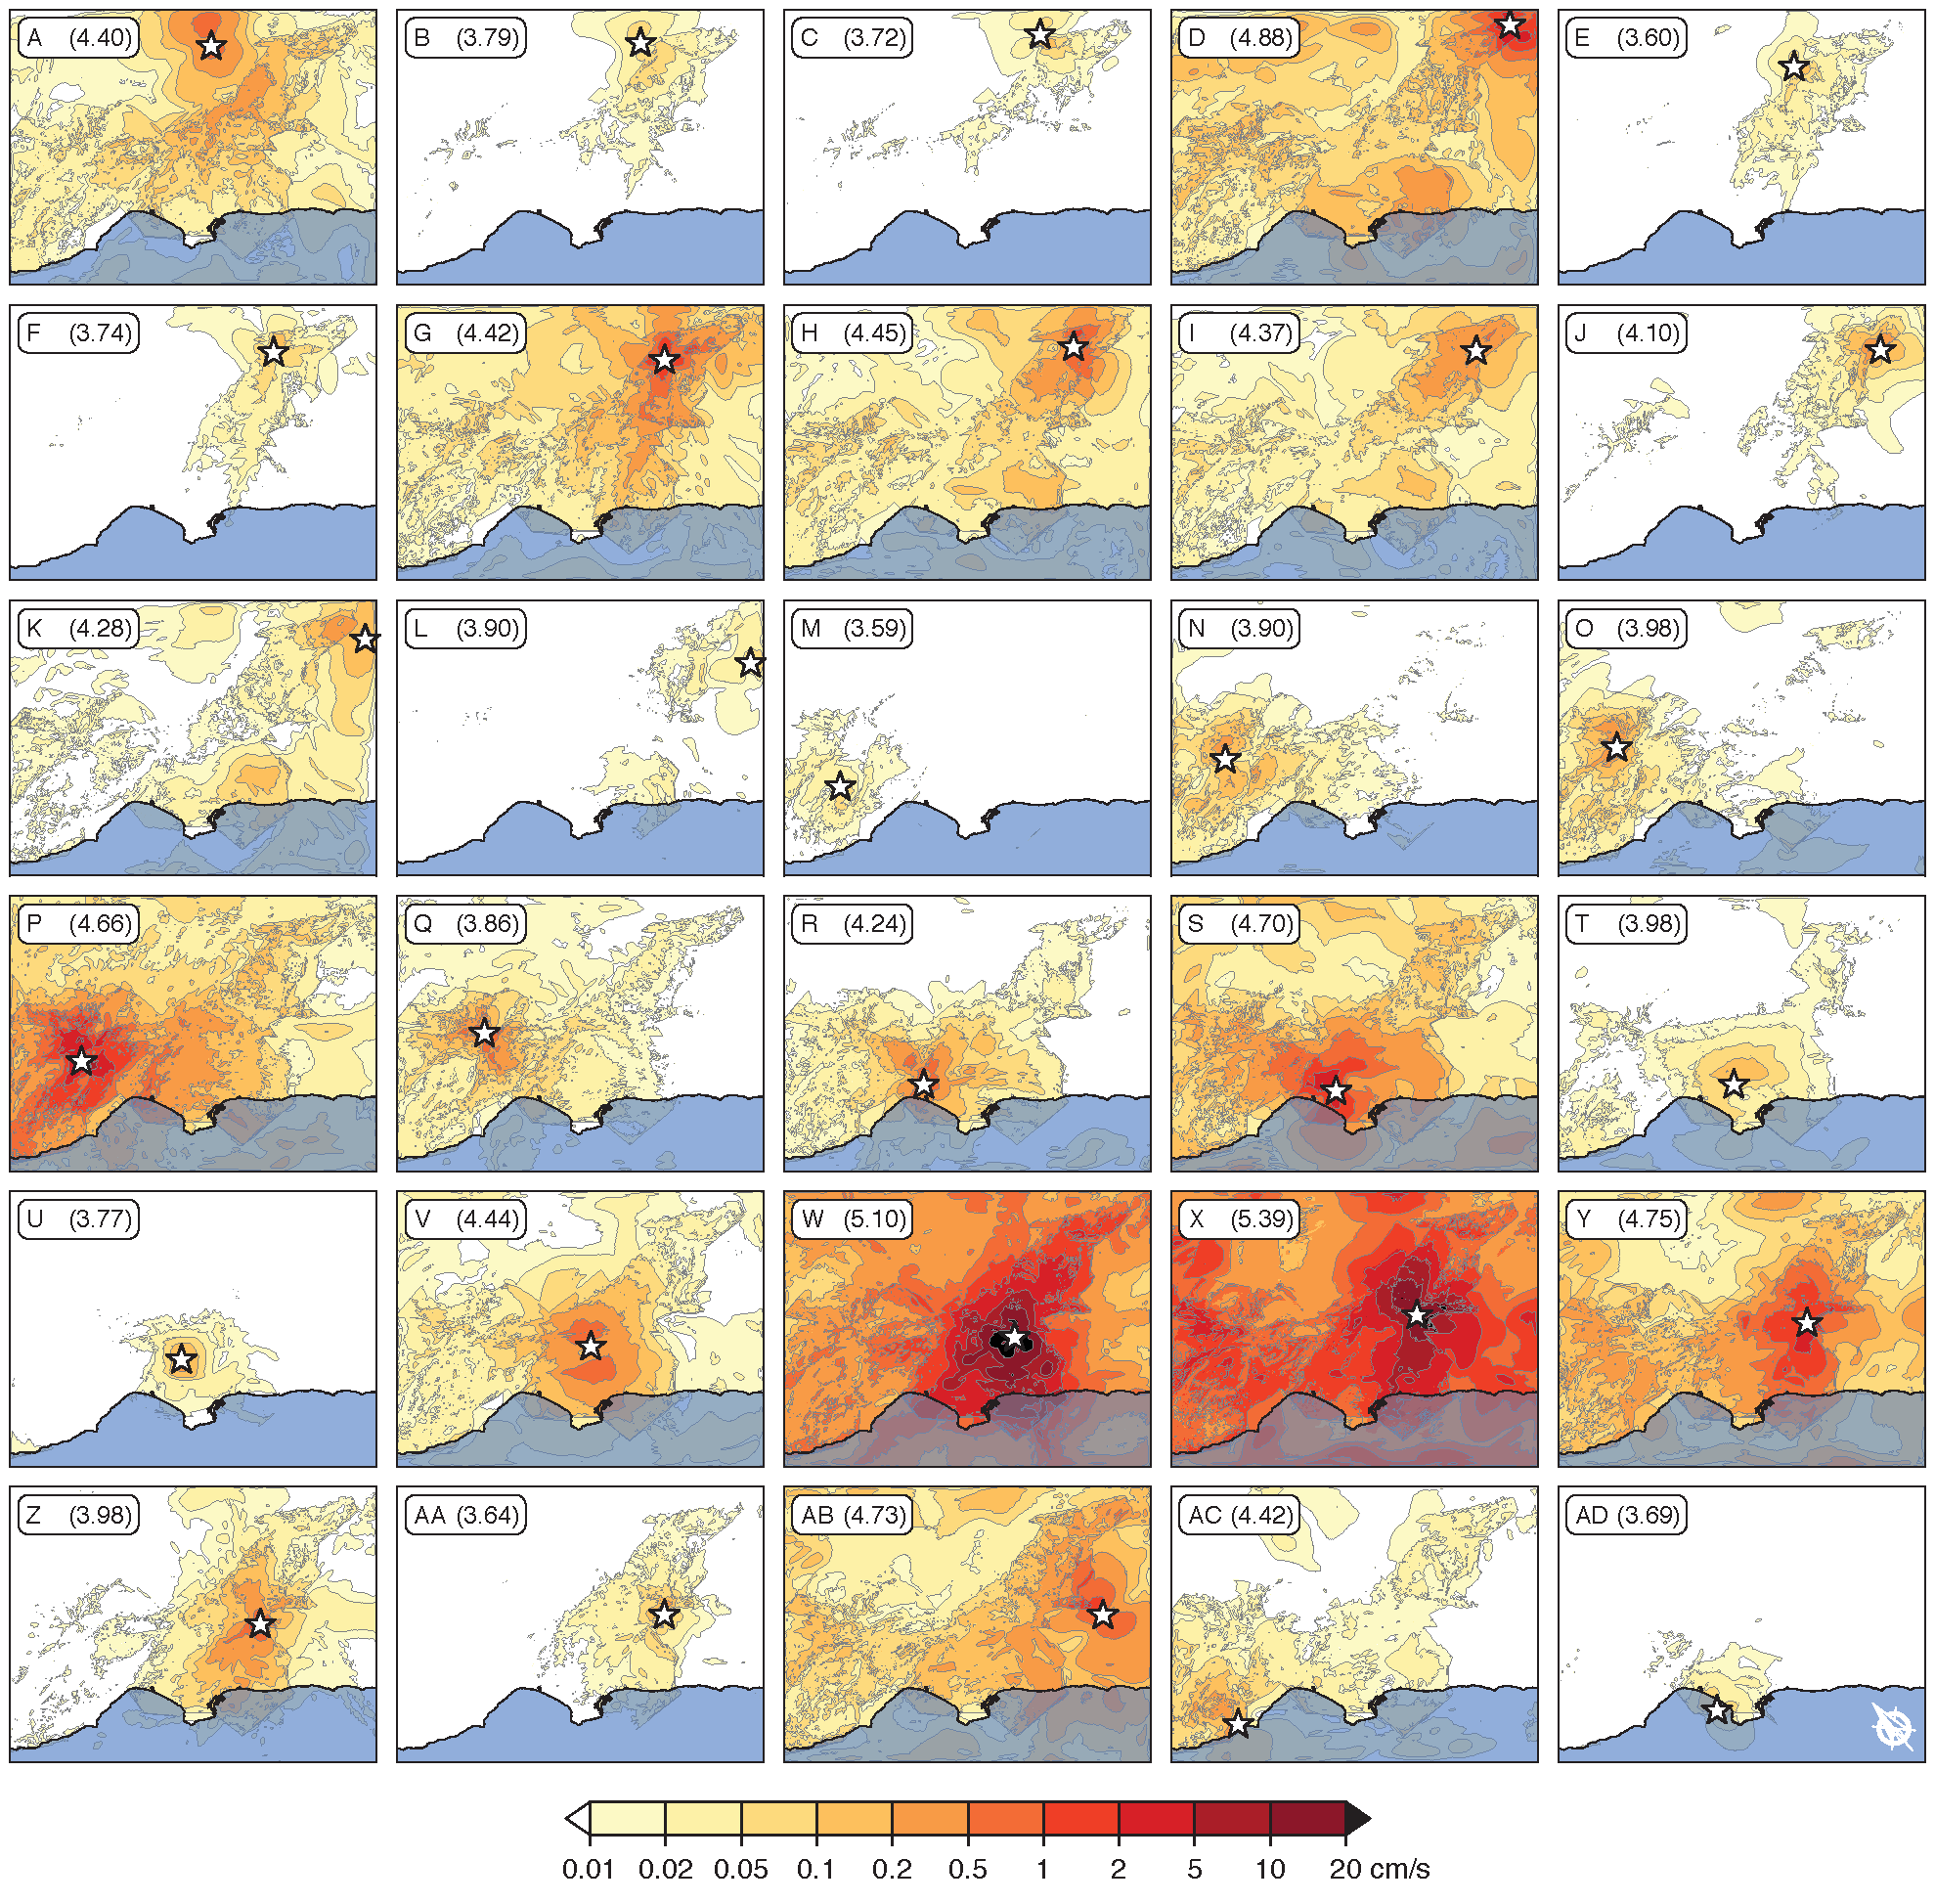
\includegraphics
        [width=\columnwidth]
        {figures/pdf/figure-03}
    \caption{Source time functions (top: slip; middle: slip-rate), and slip-rate Fourier amplitude spectra (bottom) of all the events. Slip-rate functions were computed based on the total rise time estimated from eqs~(\ref{eq:stein}) and (\ref{eq:sliprate}). The source functions of events W and X, corresponding to the 2014 La Habra and 2008 Chino Hills earthquakes, are singled out in the figure because for reference. These two events are the largest of all earthquakes considered.}
    \label{fig:slip}
\end{figure}


